\chapter{容器云资源调度模型综述}
Docker容器虚拟化是容器云集群的核心技术,但一个高效的容器编排引擎也是集群不可或缺的部分。一个好的调度器既要提现出作业调度的“公平”性,又要兼顾其性能和鲁棒性,还要能应用于实际生产环境中。在集群数据中心,可以通过应用对资源的需求感知用户部署的应用类型,通常可以划分为CPU密集、内存密集、I/O密集和网络带宽密集型应用~\cite{Peng2016Research,Shuangke2017SchedulingStrategy}。在集群上通常是多种密集型应用同时部署和运行,调度器如何进行资源分配至关重要,这使调度变得异常复杂和困难,往往不存在最优解决方案。传统虚拟机的云计算中心资源调度已有相当多的研究,针对容器集群,各大容器厂商也相继推出了几款优秀的容器编排引擎。根据其调度架构的不同可以划分为集中式调度模型、两层调度模型、共享状态调度模型,其典型代表分别是Docker Swarm、Apache Mesos、Google Kubernetes。

\section{集中式调度模型}
\subsection{集中式调度模型概述}
集中式调度通过单个调度节点处理所有任务请求,使用固定的、单一的调度算法调度全部任务。集中式调度模型中存在一个中心调度器,所有的任务都必须经过中心调度器中统一的调度算法进行调度,资源调度和任务管理都由中央调度器负责。首先,集中式调度模型将导致系统扩展性很差,集群规模不能大规模增加,而且所有的调度信息在单节点上运算,不能并行执行,这要求中央调度器的部署节点必须是高性能计算机,否则调度节点会成为性能瓶颈。其次,集中式调度很难定制用户自己的调度策略,针对特定场景下用户自定义的调度策略要融入中央调度器是一项巨大的挑战。针对集中式调度模型的不足,Google的Omega系统也进行了一定的优化,开发多种调度策略存放于中央调度器中,根据不同的调度任务选择相应的调度策略进行任务调度,这种优化在集群规模较小时能够缩短任务执行时间,起到一定的优化效果。在大规模的容器云集群上,调度策略依然存在于单个节点上,任务的精准分类和调度策略的频繁切换得不到有效解决,系统扩展性并没有本质的改善。此外,还有通过集群硬件资源静态分区来优化集中式调度模型的方法,将集中控制的资源静态划分为多个区域,计算框架分配到特定的区域执行,多个计算框架之间从物理上进行隔离。静态划分简单有效,但集群资源利用率低下,经常出现部分计算框架系统资源不足。

\subsection{Docker Swarm集中式调度模型}
Docker公司2014年发布的容器编排管理工具Docker Swarm~\cite{Jansen2016Employing,Naik2016Building} ,无需安装、易于搭建、并且拥有活跃的社区,已应用于实际的生产环境中。
\begin{figure}[H] % use float package if you want it here
	\centering
	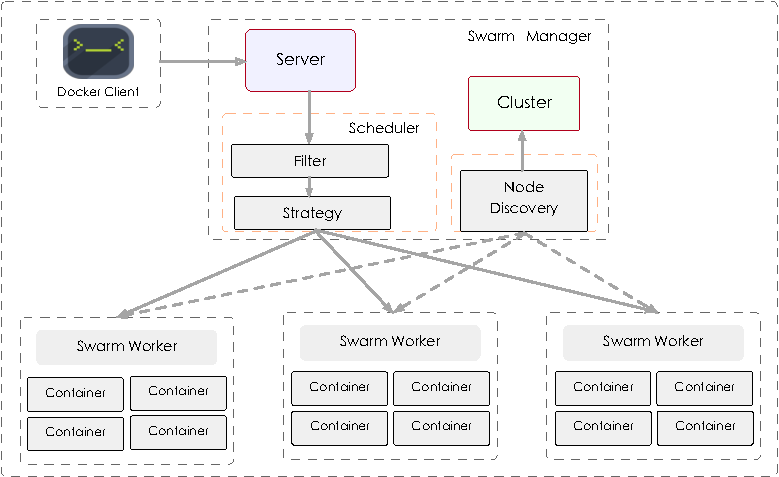
\includegraphics{swarm-structure}
	\caption{Swarm架构图\cite{Naik2016Building} }
\end{figure}

Swarm集群由管理节点和工作节点构成,其中管理节点可以配置多个,实现高可用的多管理模式,内部通过RAFT算法实现管理节点高可用性。管理节点上除Docker Daemon守护进程、Load Balancing、Scaling组件外,最为重要的是Scheduler和Discovery组件。Discovery负责集群中节点的发现和状态更新,Scheduler先根据用户的资源需求对节点进行筛选,然后使用内置的调度策略进行应用调度。工作节点主要运行Docker Daemon和Load Balancing,根据控制节点的指令运行绑定的容器应用。在调度器的过滤模块主要提供了约束过滤器和健康过滤器,此外还可以配置吸引力过滤器、依赖过滤器和端口过滤器。

约束过滤器是通过一定的约束条件筛选节点,集群中每个节点都带有一个标签Label,对于一些特殊的应用可以指定其Label标签调度到指定的节点上运行;健康过滤器过滤掉不健康的节点,避免容器调度后运行失败;吸引力过滤器是将新的容器链接到已经创建的容器上,实现共同运行和销毁,主要有镜像吸引和标签吸引两种方式。镜像吸引是将容器直接调度到拥有该镜像的节点上,避免镜像下载的重复开销,节约网络资源,标签吸引是通过标签指定链接到已创建的旧容器实现共同工作;依赖过滤器是新容器依赖于其他的容器,可能会共享磁盘卷、或在同一个网络栈上等;端口过滤器将需要特定开放端口的容器运行到开放该端口的节点上,避免容器端口不可用的情况发生	。

Swarm的调度策略的算法主要包括Random、Spread和Binpack三种~\cite{Cerin2017A},下面分别对其算法思想进行简单的介绍:
\begin{enumerate}[1.]
	\item Random算法。该算法随机从过滤完的节点中选取一个节点进行调度判断,如果该节点满足条件则将容器调度到该节点上,否则随机选取下一个节点直至找到合适的节点调度或返回调度错误信息。
	\item Spread算法是最少容器算法,该算法的初衷是保证容器集群的负载均衡。每次遍历一遍集群中每个节点上运行的容器数量,选择容器数量最少的节点进行容器调度,若该节点不满足条件,则依次从后往前进行调度尝试,直至找到满足条件的节点或返回调度错误。
	\item Binpack算法是最多容器算法,该算法的目的在于最大化利用集群中节点资源,和Spread算法相反,每次从集群中选择运行容器数量最多的节点进行容器调度,若满足条件则将容器调度至该节点,否则依次从前往后尝试调度容器到节点,直至找到合适节点或返回错误。
\end{enumerate}

\section{两层调度模型}
\subsection{两层调度模型概述}
两层调度模型是将资源调度和作业调度分开,资源调度层只负责给计算框架分配所需的资源,具体的作业调度由每个计算框架的任务调度器完成。在一些成熟的处理框架中如Hadoop、Spark、MPI等都有相对成熟和高效的调度算法,两层调度模型将这些调度算法集成进来,通过一个轻量的资源共方式来控制资源的分配和访问。如在两层调度模型上执行Hadoop处理框架,资源调度层只负责将系统资源分配给Hadoop调度框架,具体的任务调度由Hadoop自身的调度器执行。两层调度模型分而治之的设计思想极大提升了集群的可扩展性和任务调度的并行执行能力,通过中间的资源管理器为上层任务框架提供系统资源,并且掌握底层资源的全部状态。两层调度模型也存在不小的缺点,首先,上层的单个计算框架无法获取集群的全部状态,只有下层的资源调度器才掌握全部集群资源信息,这就导致上层计算框架在任务运行失败时无法做出重启还是重调度的抉择。其次,两层调度采用“悲观锁”对资源进行控制,相当于资源的一把全局锁,所有资源被推送给某个计算框架,待该计算框架系统资源分配完成后,其他计算框架才能进行资源分配,这造成系统响应慢,并发粒度小,并发性受到极大的限制。

\subsection{Apache Mesos两层调度模型}
Apache Mesos~\cite{Mesos2011}是两层调度模型中最为典型的代表,最初是加州伯克利分校的AMPLab在2009年开发的集群管理软件,用于管理快速扩张的各种分布式计算框架,后在Twitter中用于容器云集群管理,获得巨大的成功。

\begin{figure}[H] % use float package if you want it here
	\centering
	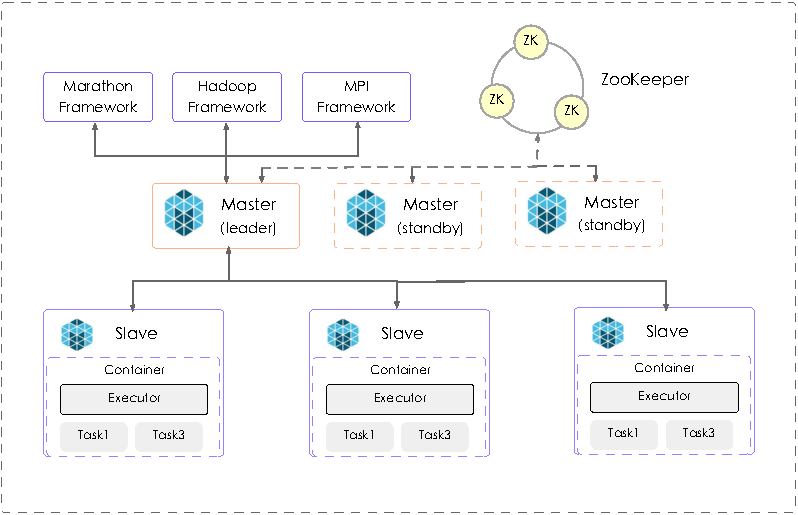
\includegraphics{mesos-structure}
	\caption{Apache Mesos架构图~\cite{Mesos2011}}
\end{figure}

如图2.2所示,Mesos的总体架构也采用主从设计,Master节点作为集群的管理控制节点,可以有一个或者多个(最好为单数),为了防止单节点故障,通过ZooKeeper提供一致性服务。每次在多个Master中选举一个作为leader对外提供服务,其他的Master副本随时保证和Master的状态一致,一旦服务出现故障,立即启用新的备份节点,从而实现集群的高可用性。集群的架构可以分为两层: 计算框架层和Master调度层。Master调度层管理众多的计算节点,负责收集各节点的资源情况并作出资源分配决定,计算框架层负责实际任务的调度。整个调度系统分为任务调度层和资源调度层,两个层级互不干扰,分别使用自身的调度算法,提升了集群调度策略的可扩展性。从架构的组成部分来看,主要有五大组成部分,下面分别对组成部分的功能进行介绍:
\begin{enumerate}[1.]
	\item ZooKeeper组件。ZooKeeper作为一款Hadoop项目中分布式系统的协调系统,主要用于解决分布式应用数据管理问题,如应用配置管理、统一命名服务、状态同步服务以及组服务和集群管理等。ZooKeeper非常简单易用、功能丰富可靠、并且提供了通用协议下开源共享的存储库,其核心就是一个精简的文件系统,还能提供一些简单和抽象的文件操作。在Mesos中,ZooKeeper主要用于解决Master节点的状态一致性和高可用问题,避免单节点故障,实现集群持续稳定的对外服务。
	\item Mesos Master组件。Master是集群的控制器,是整个集群调度的大脑中枢,既要对底层各Slave节点的资源进行收集和管理,也要通过一定的资源分配策略提供资源给上层的各处理框架Framework。当前对各Framework的资源分配策略使用DRF~\cite{DRF2011}(Dominant Resource Fairness)算法,这是一种针对多维资源(CPU、内存、I/O、网络带宽等)不同需求设计的公平调度算法。Master还负责资源的访问控制,一旦系统资源被推送给某个Framework,必须等该计算框架资源分配完成后才能再次进行其他框架的资源分配。
	\item Mesos Slave组件。该组件作为底层调度实例的具体执行者,接收来自Master的指令,将自身的资源分配给每个执行器,执行器上运行一个或多个任务,并将各任务作为容器运行起来。此外,Slave节点还定期向Master节点汇报资源使用情况作为Master调度器的调度依据。Slave上运行一个containerizer用来管理容器的生命周期,包括容器的创建、更新、监控和销毁。
	\item Framework组件。Framework负责将各计算框架如Hadoop、Spark、MPI等注册接入到集群中,Master的调度器负责对其需要的资源进行分配,具体的任务调度则由各计算框架完成。各计算框架通过调用Master的API进行任务创建和调度请求,Master再将任务下发到Slave上执行。
	\item Executor组件。Executor负责启动框架内部的Task任务,各种计算框架接入Mesos的方式,接口不同,因此要接入一个新的计算框架就需要编写一个新的Executor,用来通知Mesos如何启动框架中的Task任务。
\end{enumerate}

Mesos作为一款优秀的分布式资源管理框架,采用双层调度机制,资源分配层负责将资源分配给计算框架,计算框架使用自身的任务调度器执行任务调度。Mesos可以对集群的资源进行细粒度的划分,按照计算框架实际任务的需求进行资源分配,极大提升了集群资源利用率。Mesos不需要清楚各Framework的具体调度逻辑,只需要通过API向上提供资源分配即可,具有较强可扩展性。Mesos是模块化的实现,新增一个Framework不需要对Mesos进行重新编码,可以快速实现接入。Master节点使用ZooKeeper保证其状态一致性,能够实现高可用性。但是,Mesos对底层的资源采用“悲观锁”的方式进行控制,相当于资源的一把全局锁,所有资源被推送给某个计算框架,待该计算框架系统资源分配完成后,其他计算框架才能进行资源分配,这造成系统响应慢,并发粒度小,并发性受到极大的限制。独立的调度框架只能访问集群部分状态信息,往往不能进行调度优化。

\section{共享状态调度模型概述}
在集中式模型中,资源分配和任务管理都由中心调度器负责,并且集成了具体的调度算法,难以扩展调度策略。在两层调度模型中,资源分配由资源调度层完成,任务调度由具体的计算框架自己完成。集中式的调度很好的保证了全局状态的一致性,但是扩展性较差,两层调度虽然可扩展性较好,但并发粒度小、并行性差,并且容易造成资源的竞争和死锁。为了解决这些不足,共享状态调度模型被提了出来,其核心在于所有的调度逻辑共享集群状态,选择最优的节点进行资源分配和任务调度。
其中最为典型就是Google推出的Borg~\cite{KUB2015}、Kubernetes以及使用事务方式解决一致性管理问题的Omega~\cite{Burns2016Borg},其中Kubernetes以其轻量开源的特点深受大家喜爱,各大主流的互联公司都加大了对其支持力度。

\begin{figure}[H] % use float package if you want it here
	\centering
	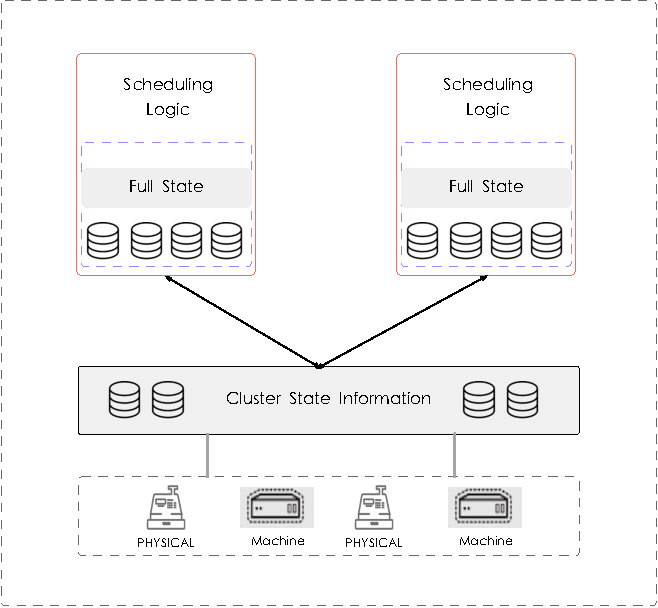
\includegraphics{full-state-structure}
	\caption{共享状态资源调度模型~\cite{Burns2016Borg}}
\end{figure}
在共享状态调度模型中,每一个上层的调度器都可以对整个集群的状态进行访问,资源对所有的调度器都是透明的,可以进行自由竞争,不存在单一的资源分配器,也不存在单一节点访问瓶颈。集群不仅支持节点资源的快速增加,也支持调度器的扩展,用户根据自己的实际应用场景开发特殊的调度器,并且很轻易地集成到系统中。为保证集群的高并发性和可扩展性,共享状态调度模型采用“乐观锁”~\cite{Halici1991An}对底层资源进行并发控制。具体的实现是通过对集群的所有状态都增加一个版本属性,每次提交时比较提交的版本和当前数据版本号大小,若版本号小于当前的版本号,则不进行任何处理,只有提交版本号大于当前数据版本号的操作才被接受,更新完状态后版本号递增。“乐观锁”并发控制虽然会增加资源访问的冲突数,影响系统的吞吐率,但在实际的系统中依然在一个可以接受范围,下一小节将对Kubernetes调度模型架构和流程做详细的分析。

\section{Kubernetes共享状态调度模型}
Kubernetes是典型的基于共享状态的调度模型,是一个轻量开源的平台,用于容器应用管理和服务,使用Label和Pod的概念将容器划分为逻辑单元,实现关联容器共同部署和调度。本小节对Kubernetes核心组件和整体架构进行深入研究,尤其是分析其调度算法的不足,为下一步提出新的调度方案提供依据。
\subsection{Kubernetes简介}
Kubernetes源自Google的Borg项目,Borg是Google集群管理工具,一直用于管理全球上百万台服务器,性能稳定可靠。为在容器云竞争中占据主导地位,Google基于Borg的管理经验,研发了Docker的容器编排工具Kubernetes,并在2014年将其开源,逐步发展成为一个大的生态技术圈。作为一个跨主机的应用容器编排引擎,Kubernetes提供了一系列强大的功能,包括应用容器部署、资源调度、服务发现、动态扩容以及错误恢复等。Kubernetes强大的集群管理能力非常适用于分布式系统,实现了多租户应用、服务发现、服务注册、负载均衡、故障发现和自动恢复、在线扩容、细粒度调度、资源配额管理等功能,完美定义了构建业务系统的标准化架构。除集群管理方面强大功能外,Kubernetes还提供完整的开发、测试、部署、发布、运维监控等各种开发管理工具。

Kubernetes逐步发展成一个巨大生态圈,为容器编排提供一种简单、轻量的方式,用户还可以进行功能定制。采用Kubernetes的云计算服务商和用户越来越多,如微软、Yahoo、IBM、华为、VMware、网易、阿里、百度等,还有一些初创公司灵雀云、青云等都采用Kubernetes作为容器云的管理系统。

Kubernetes拥有强大而活跃的社区,众多开发者不断对其进行迭代更新,其代码更加完善。当前Kubernetes社区的支持者有Google、CoreOS、RedHat、华为、网易、阿里云、浙大SEL实验等。Google在2015年联合其他20多家公司成立了开源组织CNCF(Cloud Native Computing Foundation),加入OpenStack社区,致力于Kubernetes的应用推广,支持其在公有云、私有云等更多基础设施平台上应用,提供更加简便丰富的工具集,方便用户开发和使用。

\subsection{Kubernetes架构和组件}
Kubernetes是一个主从架构体系,该集群管理器很好地解决了扩容和服务升级两大难题,具有较强的横向扩展能力,Kubernetes的整体架构图~\cite{KUBdoc}如下。
\begin{figure}[H] % use float package if you want it here
	\centering
	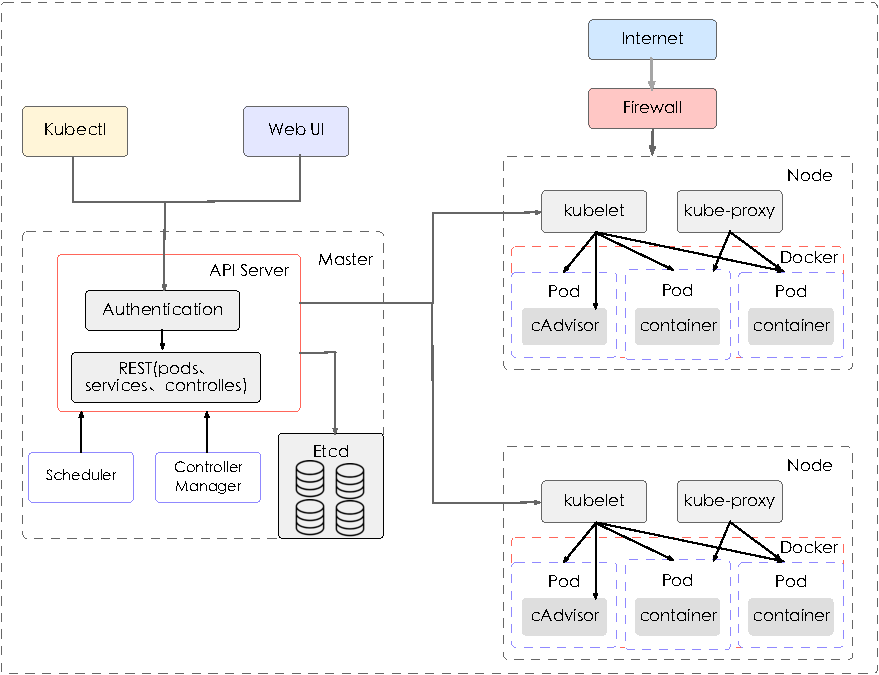
\includegraphics{kubernetes-structure}
	\caption{Kubernetes体系架构图~\cite{KUBdoc}}
\end{figure}
如图2.4所示,Kubernetes主从架构主要由控制节点Master、工作节点Node以及外部工具集kubectl、web UI等附加依赖组成。Master作为集群的控制节点,主要负责集群的管理调度,由API Server、Scheduler、Etcd、Controller Manager等组成,实现其主要功能。Node节点主要根据控制节点的指令执行具体的任务,实现应用容器的运行,主要由kubelet、kube-proxy、cAdvisor、Container Runtime等组成。外部可以通过kubectl命令工具对集群进行增删查改的操作,也可以使用Web UI与集群进行交互。下面对集群中的重要组件分别进行介绍:
\begin{enumerate}[1.]
	\item  API Server组件。API Server是系统管理指令的统一入口,负责对外提供RESTful的API服务功能,所有与集群的交互都需要通过API Server组件完成,是集群外部和内部的通信枢纽。APIServer也是资源配额限制的入口,通过Authentication组件提供集群完备的安全认证机制。API Server接收外部Web browser或kubectl的命令请求,将REST对象和状态持久化到Etcd中存储,同时与Node节点上的kubelet进行交互。
	\item Scheduler组件。集群调度组件,负责集群资源调度和Pod分配工作,Scheduler监控集群中未分配的Pod,根据其对资源的约束条件和集群资源可用性,将Pod调度到实际的Node上运行。调度器是一个可插拔的模块,用户可以开发自己的调度算法集成到集群中,其调度流程和调度策略后面会详细介绍。
	\item Controller Manager组件。控制管理器提供服务发现、集群管理、Pod扩容、服务绑定、应用生命周期管理等功能。其中Node Controller用于管理节点、Replication Controller用于应用容器管理,保证容器副本和需求一致、Namespace Controller用于命名空间管理、Service Controller提供负载和服务代理、Persistent Controller管理维护Persistent Volume和Persistent Volume Claim等。
	\item Etcd组件。一个高可用、强一致性的服务发现键值存储仓库,用于保存集群中所有的网络配置和对象的状态信息,具有中心数据库的地位,进行分布式的部署,通过watch机制进行服务更新支持。
	\item Kubelet组件。Kubelet是运行在Node节点上的控制器,用于裁决和驱动容器的执行层,是API Server和Pod的主要实现者。单个Pod中可以运行多个容器和存储数据卷,能够将Pod和相关的依赖项很方便地打包迁移,	API Server进行访问控制,Scheduler进行资源的调度,但是最终Pod能否在Node上运行成功是由kubelet决定的。此外,kubelet通过cAdvisor组件对Node节点的状态、资源进行监控,定期汇报给控制节点,存储在Etcd中。
	\item Kube-Proxy组件。负责负载均衡和反向代理组件,通过创建Pod的代理服务,用户可以通过IP地址直接访问Pod应用,实现服务到Pod的路由转发。此外,kube-proxy还实现了一个高可用的负载均衡解决方案。
\end{enumerate}

除上述给出的核心组件外,Kubernetes还有负责提供集群DNS服务的kube-dns、提供外网访问入口的Ingress Controller、提供资源监控的Heapster、提供管理控制界面的Dashboard、提供日志采集、存储和查询的Fluentd-elasticsearch组件等。

\subsection{Kubernetes任务处理流程}
Kubernetes调度器运行在Master节点上,作为一个可插拔的模块,在默认配置下,调度器可以满足大部分的需求,如特定的Pod分配到指定的节点,相同集合下的Pod分配到不同节点,平衡各节点的资源使用率等。但在一些特殊的应用场景下,尤其涉及多计算框架容器应用对大数据的处理,其默认配置的调度方法显得力不从心,需要用户开发自己的调度策略。
\begin{figure}[H] % use float package if you want it here
	\centering
	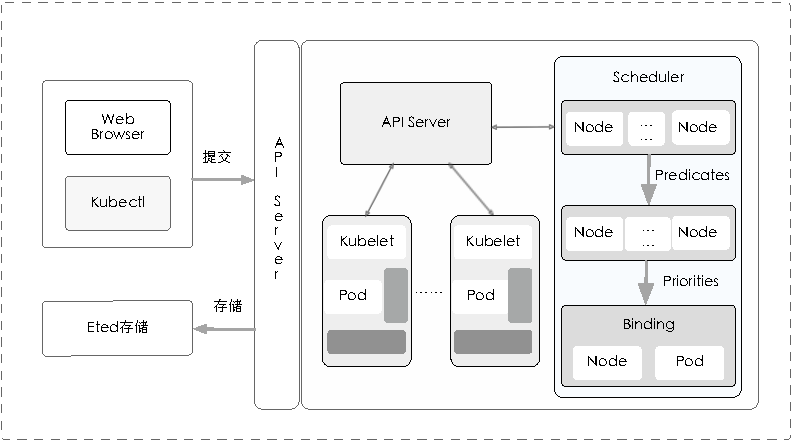
\includegraphics{kubernetes-scheduler}
	\caption{kubernetes任务处理流程~\cite{KUBdoc}}
\end{figure}
调度器相对于普通用户而言类似一个黑盒,输入Pod的资源需求,输出Pod和节点的绑定策略,起到指挥中枢的作用。但是在很多业务场景下,用户希望自己的Pod调度可控,如定制调度算法、特殊硬件需求的Pod调度到相应的节点、通信量大的计算框架部署在相同区域和机架、数据需求大的Pod部署在数据节点等。Kubernetes的任务处理流程如图2.5所示,命令工具Kubectl或Web Browser向Master上的API Server发送任务请求如创建Pod,API Server对请求做出响应处理并将处理的结果和状态存储在Etcd中,同时设置PodSpec.NodeName为空,加入未调度Pod队列。调度器监控Etcd中未调度Pod队列状态,发现有未调度的Pod时通过调度策略尝试绑定Pod 到满足需求的节点。调度策略将满足资源需求的节点进行综合评分,主要考虑资源使用的均衡性、相同副本的容灾性等因素,最终选取得分最高的节点,将Pod调度到该节点上,并将绑定状态存储到Etcd中。节点上的Kubelet监控Etcd中Pod调度结果,接管任务的后续工作,负责Pod生命周期的管理,一个完整的任务处理流程结束。

\section{本章小结}

本章主要介绍基于Docker构建的三种典型容器调度模型: 集中式调度模型、两层调度模型和共享状态调度模型,并以Docker Swarm、Apache Mesos和Kubernetes为例对比分析三种调度模型的组织架构和调度优缺点,最后重点分析了容器编排引擎Kubernetes共享状态调度模型的任务处理流程和调度原理,为提出新的共享状态调度方法奠定基础。




